\documentclass[papersize=a4]{report}
\usepackage{graphicx, amsmath, amsthm, amssymb, listings, multirow, wrapfig, floatrow}
\usepackage{tikz}
\usetikzlibrary{arrows}

\usepackage{color} %red, green, blue, yellow, cyan, magenta, black, white
\definecolor{mygreen}{RGB}{28,172,0} % color values Red, Green, Blue
\definecolor{mylilas}{RGB}{170,55,241}
\usepackage[a4paper, left=26mm, right= 26mm, top=35mm ]{geometry}
\usepackage{xepersian}
\usepackage{setspace}
\settextfont[Scale=1]{XB Niloofar}
\setdigitfont[Scale=1]{Yas}


\newcommand{\R}{\mathbb{R}}
\newtheorem{theorem}{قضیه}
\renewcommand{\chaptername}{سوال}

\newcommand{\bigCI}{\mathrel{\text{\scalebox{1.07}{$\perp\mkern-10mu\perp$}}}}

\title{استنتاج علّی\\تمرین کامپیوتری اوّل}
\author{بهراد منیری \\ ۹۵۱۰۹۵۶۴}
\date{\today}

\begin{document}
\doublespacing
\maketitle
\chapter{}	
\section{بخش الف}

\begin{enumerate}
	\item 	\textbf{مدل خطی با نویز گاوسی}
	$$
	X \rightarrow Y :
	\begin{cases}
	X := N_x\\
	Y := X + N 
	\end{cases}
	N \bigCI N_x
	$$
	با توجه به این موضوع داریم
	$$\forall \alpha, \beta: \;\;  \alpha X + \beta Y = Normal \rightarrow (X, Y): Multi\;Variable\;Normal$$
	در نتیجه توزیع‌های مارجینال و شرطی نیز همگی نرمال هستند.
$$
\begin{cases}
P(Y|X=x) = \textrm{Normal}(x, \sigma_N)\\ 
P(X|Y=y) = \textrm{Normal}(-\frac{y}{2}, \sigma_N)
\end{cases}
$$
این توزیع ها در شکل 
\eqref{1}
رسم شده‌اند.

	
\item 	\textbf{مدل غیرخطی با نویز گاوسی}

$$
X \rightarrow Y :
\begin{cases}
X := N_x\\
Y := X + 5X^3 + N 
\end{cases}
N \bigCI N_x
$$


این توزیع ها در شکل 
\eqref{2}
رسم شده‌اند.

	\begin{figure}
		\centering
			\includegraphics[scale=0.35]{lin_cond1.png}
		\begin{floatrow}

			\includegraphics[scale=0.35]{lin_cond2.png}
			\includegraphics[scale=0.35]{lin_cond3.png}
		\end{floatrow}
		\caption{توزیع‌ها با فرض 	$\sigma_x = \sigma_N = 0.5$	}
		\label{1}
	\end{figure}

	\begin{figure}
		\centering
		\includegraphics[scale=0.35]{non_con1.png}
		\begin{floatrow}
			\includegraphics[scale=0.35]{non_cond2.png}
			\includegraphics[scale=0.35]{non_cond3.png}
		\end{floatrow}
		\caption{توزیع‌ها با فرض 	
			$\sigma_x =1,\;\; \sigma_N = 10$}
		\label{2}
	\end{figure}
	
\end{enumerate}
\section{بخش ب}
\section{بخش ج}
\subsection{دیتاست آبفشان}

ابتدا داده‌ها را در یک فضای دو‌بعدی رسم می‌کنیم تا شهود بهتری نسبت به مسأله پیدا کنیم، شکل \eqref{abfeshan}.
\begin{figure}[h]
	\centering
	\includegraphics[scale=0.45]{old1.png}
	\caption{رسم دیتای مربوط به آبفشان}
	\label{abfeshan}
\end{figure}

برای تشخیص جهت درست علّیت،  با فرض \lr{ANM}، مطابق بخش‌های قبل یک‌بار هر یکی از دو متغیّر را علّت فرض کرده و رگرسیون‌های غیرخطی مربوط را انجام می‌دهیم.  
$$
\begin{cases}
Y = \hat{f_1}(X) + \hat{N}_1 &\;  :X \rightarrow Y \text{با فرض}  \\
X = \hat{f_2}(Y) + \hat{N}_2 &\;  :Y \rightarrow X \text{با فرض}
\end{cases}
$$
انتظار داریم که در جهت درست علّیت، N و متغیّری که عنوان علّت در نظر گرفته‌ایم مستقل شوند. با انجام این فرآیند در هر دو جهت و اعمال آزمون استقلال هیلبرت-اشمیت برای دو کمیت مذکور در هر جهت، جهت درست علّیت را تشخیص می‌دهیم.

شکل \eqref{erup} رگرسیون با فرض اینکه زمان فوران کنونی علّت فاصله‌ی زمانی تا فوران بعدی است و شکل \eqref{wait} نیز رگرسیون با فرض معکوس است.
\begin{figure}[h]
	\begin{floatrow}
	\centering
	\includegraphics[scale=0.451]{erup_time1.png}
	\includegraphics[scale=0.451]{erup_time2.png}
	\end{floatrow}
	\caption{رگرسیون با فرض اینکه زمان فوران کنونی علّت فاصله‌ی زمانی تا فوران بعدی است.}
	\label{erup}
\end{figure}

\begin{figure}[h]
	\begin{floatrow}
		\centering
		\includegraphics[scale=0.451]{waiting_time1.png}
		\includegraphics[scale=0.451]{waiting_time2.png}
	\end{floatrow}
	\caption{رگرسیون با فرض اینکه فاصله‌ی زمانی تا فوران بعدی علّت زمان فوران کنونی است.}
	\label{wait}
\end{figure}
با این کار و انجام آزمون فرضیه‌ی \lr{HSIC}، متوجه می‌شویم با فرض 
\textbf{«زمان فوران کنونی علّت فاصله‌ی زمانی تا فوران بعدی است» }
زیرا همان‌طور که در شکل \eqref{erup} دیده‌ می‌شود، بعد از رگرسیون فاصله‌ی زمانی تا فوران بعدی بر حسب طول زمان فوران فعلی، مقدار residue این رگرسوراز فاصله‌ زمانی فوران فعلی مستقل است. این موضوع تا حدی بدیهی است زیرا فوران بعدی، بعد از فوران فعلی رخ داده و نمی‌تواند تاثیر علّی بر فوران فعلی داشته باشد.

\subsection{دیتاست صدف}
در این دیتاست قصد داریم جهت علّی بین طول این نوع صدف و تعداد حلقه‌های آن را پیدا کردیم. می‌دانیم که تعداد حلقه‌ها رابطه‌ای تقریباً غیرتصادفی با سن  صدف دارد. از نظر شهودی،‌ سن صدف(یا به عباری تعداد حلقه‌ها) علّت طول صدف است. در این بخش این موضوع را به کمک دیتای داده‌شده تایید می‌کنیم.
یک بار با فرض سن صدف(یا به عباری تعداد حلقه‌ها) علّت طول صدف، الگوریتم را اجر می‌کنیم. شکل 
\eqref{cor}
نتایج این کار هستند. شکل 
\eqref{wrong}
نیز نتایج اجرای الگوریتم با فرض طول صدف علّت تعداد حلقه‌ها (یا به عبارتی سن صدف) هستند.
\begin{figure}[h!]
	\centering
	\begin{floatrow}
		\includegraphics[scale=0.4]{aba_for1.png}
		\includegraphics[scale=0.4]{aba_for2.png}
	\end{floatrow}
\caption{ سن صدف(یا به عباری تعداد حلقه‌ها) علّت طول صدف}
\label{cor}
\end{figure}

\begin{figure}
	\centering
	\begin{floatrow}
		\includegraphics[scale=0.4]{aba_back1.png}
		\includegraphics[scale=0.4]{aba_back2.png}
	\end{floatrow}
\caption{طول صدف علّت تعداد حلقه‌ها (یا به عبارتی سن صدف)!}
\label{wrong}
\end{figure}
با توجه این نتایج و اعمال آزمون استقلال و همچنین با توجه به نمودارهای residue بر حسب متغییر علّت فرض شده، فرض ما مبنی بر اینکه
\textbf{سن صدف(یا به عباری تعداد حلقه‌ها) علّت طول صدف}
تایید می‌شود. 
%%%%%%%%%%%%%%%%%%%%%%%%%%%%%%%%%%%%%%%%%
\chapter{}

می‌دانیم داده‌های این سوال از یک SCM تولید شده‌اند و اسکلت گراف این SCM در شکل روبروآمده است. حال سعی می‌کنیم با چند بار تکرار فرایندی که در سوال قبلی طی شد، در این سوال نیز جهت‌‌های درست گراف را تشخیص دهیم.  این کار را در چند مرحله انجام می‌دهیم. یعنی با فرض‌های مختلف علّیت، رگرسیون انجام داده و چک می‌کنیم که آیا residue این رگرسیون مستقل از علت‌های مفروض هست یا خیر. در جهت درست علیّت این شرط برقرار است.

\begin{figure}
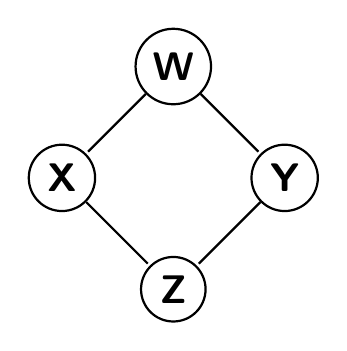
\begin{tikzpicture}[-,>=stealth',shorten >=1pt,auto,node distance=2cm,
thick,main node/.style={circle,draw,font=\sffamily\Large\bfseries}]
\node[main node] (w) {W};
\node[main node] (x) [below left of=w] {X};
\node[main node] (z) [below right of=x] {Z};
\node[main node] (y) [below right of=w] {Y};
\path[every node/.style={font=\sffamily\small}]
(w) edge node [left] {} (x)
(w) edge node [left] {} (y)
(y) edge node [left] {} (z)
(x) edge node [left] {} (z);
\end{tikzpicture}
\label{skeleton}
\caption{اسکلت گراف مربوط به داده‌ها}
\end{figure}
\vspace{0.1cm}
\begin{itemize}
	\item	\textbf{ تعیین جهت یال‌های متصل به Z}	
	در صورتی که فرض کنیم هر دو یال به این راس وارد می‌شود و رگرسیون
	$z = \hat{f} (x, y) + \epsilon$
	را حساب کنیم، دیده‌می‌شود که داریم:
	$$\epsilon \bigCI X, \; \;\; \epsilon \bigCI Y$$
	که این نشان می‌دهد این، جهت درست علیّت است. با فرض‌های دیگر، نتایجی مخالف انتظارمان از جهت درست علیّت بر خواهیم داشت.
در شکل
\eqref{forward}
فرض شده است که $X \rightarrow Z \leftarrow Y$	و در شکل 
\eqref{back}
فرض شده 
$X \rightarrow Z \rightarrow Y$.
دیده می‌شود در تمام حالت به جز شکل
\eqref{forward}
تست‌های استقلال نتایجی سازگار با گراف ندارند و بنابراین حالت 
\eqref{forward}
را به عنوان حالت صحیح می‌پذیریم.

\begin{figure}[h]
	\includegraphics[scale=0.455]{b1.png}
	\label{forward}
	\caption{
		مقدار Residueی
		 $Z = \hat{f}(X,Y)$
		بر حسب X و Y با فرض 
		$X \rightarrow Z \leftarrow Y$	
}
\end{figure}

\begin{figure}[h]
	\includegraphics[scale=0.455]{b2.png}
	\label{back}
	\caption{
		مقدار  Residue ی
		$Z = \hat{f}(X)$
		بر حسب X با فرض 
		$X \rightarrow Z \rightarrow Y$	
	}
\end{figure}


	\item	\textbf{تعیین جهت یال‌های متصل به W}	
ابتدا فرض می‌کنیم که هر دو یال از W خارج شوند. \\با این فرض برای X و Y داریم
$$
\begin{cases}
X := f_1(W) + N_x\\
Y := f_2(W)  + N_y
\end{cases}
W \bigCI N_x, \;\; W \bigCI N_y
$$
حال سعی می‌کنیم این SCM را بر دیتای داده شده برازش کنیم. با انجام دو رگرسیون و بررسی استقلال Residue از علّت، به نتایج زیر می‌رسیم.
\begin{figure}
	\centering
	\begin{floatrow}
		\includegraphics[scale=0.45]{WtoX.png}
		\includegraphics[scale=0.45]{WtoY.png}
	\end{floatrow}

\caption{
مقدار Residue ی
$ Y=\hat{f}(W) $
و
$ X = \hat{g}(W)$
  بر حسب $W$ با فرض
$ Y \leftarrow W \rightarrow X$
}
\label{Forward}
\end{figure}


این تنها حالتی است که با 
\lr{Confidence Level}
دو درصد، تمام تست‌های استقلال منجر به نتیجه‌ی مورد نظرمان می‌شوند. 
شکل
\eqref{backward}
  یک فرض اشتباه است که در نهایت، Residue  ها از کمیّت‌هایی که علت ‌$W$ در نظر گرفته شده‌اند مستقل نشده است.

\begin{figure}[h]
\centering
\begin{floatrow}
	\includegraphics[scale=0.45]{back1.png}
	\includegraphics[scale=0.45]{back2.png}
\end{floatrow}

\caption{
مقدار Residue ی 
$W = \hat{f}(X, Y)$
بر حسب $X$ و $Y$ با فرض 
$Y \rightarrow W \leftarrow X$
}
\label{backward}
\end{figure}
\end{itemize}


با توجه به دو مشاهده‌ی فوق، با فرض گراف زیر، تمام آزمون فرضیه‌های استقلال مربوطه با
\lr{Confidence Level}
دو درصد نتیجه‌ای سازگار هستند.

\begin{figure}[h]
	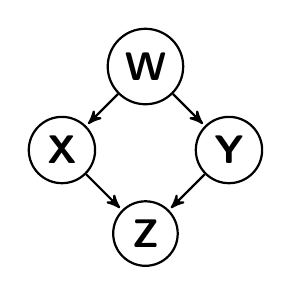
\begin{tikzpicture}[->,>=stealth',shorten >=1pt,auto,node distance=1.5cm,
	thick,main node/.style={circle,draw,font=\sffamily\Large\bfseries}]
	\node[main node] (w) {W};
	\node[main node] (x) [below left of=w] {X};
	\node[main node] (z) [below right of=x] {Z};
	\node[main node] (y) [below right of=w] {Y};
	\path[every node/.style={font=\sffamily\small}]
	(w) edge node [left] {} (x)
	(w) edge node [left] {} (y)
	(y) edge node [left] {} (z)
	(x) edge node [left] {} (z);
	\end{tikzpicture}
	\caption{گراف نهایی}
	\label{final}
\end{figure}


\end{document}